%-----------------------------------------------------------------------------------------
%
% This template has designed by Mohamad Khaleqi
% You're very welcome to edit and use this template
% 2015-02-26
% Swansea University
%
%----------------------------------------------------------------------------------------

\documentclass[a4paper,10pt]{article}
\usepackage[utf8]{inputenc}
\usepackage[toc,page]{appendix}
\usepackage{fancyhdr} % Required for custom headers
\usepackage{lastpage} % Required to determine the last page for the footer
\usepackage{extramarks} % Required for headers and footers
\usepackage{graphicx} % Required to insert images
\graphicspath{ {resources/} }
\usepackage{comment} % Comment
\usepackage[english]{babel}
\usepackage[utf8]{inputenc} 
\usepackage{url} % URL in Footnote  
\usepackage{cite} % BibLatex
\usepackage{babel,blindtext} %produce some bloody text
\usepackage{listings}
\usepackage[table]{xcolor}
\usepackage{csquotes} %Quotation
\usepackage[document]{ragged2e} % Justify

%--------------------Not needed 
%\usepackage[backend=bibtex]{biblatex}
%\bibliography{Assignment_2.bib}

\usepackage{float}
\usepackage{courier}
\usepackage{todonotes}
\usepackage{hyperref}
\usepackage{glossaries}
\makeglossaries

% Margins
\topmargin=-0.45in
\evensidemargin=0in
\oddsidemargin=0in
\textwidth=6.5in
\textheight=9.0in
\headsep=0.25in 


\linespread{1.1} % Line spacing


%----------------------------------------------------------------------------------------
%	TITLE SECTION
%----------------------------------------------------------------------------------------
\newcommand{\horrule}[1]{\rule{\linewidth}{#1}} % Create horizontal rule command with 1 argument of height
\title{
\normalfont \normalsize 
\begin{LARGE} \textsc{Swansea University} \end{LARGE} \\ [15pt] % Your university, school and/or department name(s)
\begin{large} \textsc{Computer Science} \end{large} \\ [15pt] % Your university, school and/or department name(s)
\vspace{50px}
\horrule{0.5pt} \\[0.4cm] % Thin top horizontal rule
\begin{Huge}Software Requirements Specification \end{Huge}% The assignment title
\horrule{2pt} \\[0.5cm] % Thick bottom horizontal rule
}
\author{} % Your name
\date{} % Today's date or a custom date


%------------------------------------------------------------------------------------
% Document begin
%------------------------------------------------------------------------------------
\begin{document}
\pagenumbering{gobble} %stop page number
%------------------------------------------------------------------------------------
% Page Title
%------------------------------------------------------------------------------------
\begin{titlepage}
\begin{figure}
  \centering
	
\includegraphics[width=4cm]{swantech_chess_logo}
\end{figure}
\maketitle
%\center \begin{LARGE} Software Technology Project Development, CS-M40\\ \end{LARGE}
\vspace{50px}
\begin{flushleft}
  \textit{Mohamad \textsc{Khaleqi}, 808956} \\
  \textit{Ifetayo \textsc{Agunbiade}, } \\
 \textit{Simon \textsc{Hewitt}, 806068} \\
  \hfill Customer/ Lecturer / Marker \textit{Dr. Ben \textsc{Mora}}
\end{flushleft}
\vfill
\center \date{\normalsize February 2015} % Today's date or a custom date

\end{titlepage}
\pagebreak


\pagenumbering{arabic} %start page number
%------------------------------------------------------------------------------------
% Table of content
%------------------------------------------------------------------------------------
\tableofcontents
\pagebreak
\justify

%------------------------------------------------------------------------------------
% Document begin
%------------------------------------------------------------------------------------

\renewcommand{\abstractname}{Revision History}
\begin{abstract}
\begin{center}
  \begin{tabular}{ |  p{3cm} | p{3cm} |  p{5cm} | p{2cm} |}
    \hline
    Name & Date & Reason of changes & Version \\ \hline \hline
    Simon Hewitt & 28/3/15 & Added Requirements & 0.1 \\ \hline 
    Team & 9/3/15 & All sections complete & 0.2 \\
    \hline
  \end{tabular}
\end{center}
\end{abstract}


\setlength{\parindent}{0cm}

%-----------------------------------------------------------------------------------------
% Introduction
%-----------------------------------------------------------------------------------------
\section{Introduction}
\subsection{Purpose}

This document describes the creation of an interactive Chess game by the authors as the submission for module \textbf{M24 Software Team Project}, an element of the MSc in Computer Science at Swansea University.

The Chess game requirements are described in the project assignment \cite{Assignment2Spec}, this document formalises those requirements and clarifies them with derived requirements or by open issues. 

\subsection{Document Conventions}

Code extracts are shown in \texttt{Courier mono-spaced font}


\subsection{Intended Audience and Reading Suggestions}

This document is intended for two audiences, the customer commissioning the game application, Dr Ben Mora, and for the developers and testers charged with creating the app. It is necessary to be familiar with \cite{Assignment2Spec} to fully understand and utilise this document. 

\subsection{Product Scope}

The product, a game application, is intended to be a relatively simple and entry-level chess game that is none the less fully functioning and useable by beginner or expert Chess players. By using an open source Chess engine we expect to be able to provide a challenging game to expert players. By providing a network capability, we can provide the opportunity for two players to play at a remote distance, for instance while both attending different lectures. 

\subsection{References}
References are listed at the end of the document.

All documentation related to this project are available on GitHub as a public repository:\\
\textbf{https://github.com/csm24/CS-M24}\\
In particular the minutes of meetings and Java source code used to create the UI mock-ups are available here. 

%-----------------------------------------------------------------------------------------
% Overall Description
%-----------------------------------------------------------------------------------------
\section{Overall Description}
\subsection{Product Perspective}
It should be born in mind that this product is created in a single module undertaken in one semester of our MSc course, so cannot expect to be as comprehensive or as polished as the many free and commercial chess games available. However we hope to produce an attractive game that can be played by beginner through to expert level Chess players.

\subsection{Product Functions}

The Chess game is started by a human User. When starting a new game, the user can select to play herself, against another human player, or against a computer Chess Engine, or against another instance of this app that is available on an IP network. Or she can select for the Chess Engine to play itself or to play a network player (which in turn could be a human or an engine). 

The game app has the expected usual functions of Player profiles including games won and lost, a live Game score, and a game list so the user can review the most recent game. 

\subsection{User Classes and Characteristics}
This simple game app has only a single class of User, the game player. There are no administrative functions requiring elevated security. 

\subsection{Operating Environment}


\section{Environment}


The team members use different desktop OS including Linux, OS X and Windows, so tools must support each of these. The software development tools will be:    \\

\setlength\extrarowheight{5pt}
\begin{tabular}{ || p{35mm}|p{40mm}|p{85mm} ||}

\hline
\textbf{Component} & \textbf{Selection} & \textbf{Justification} \\
\hline

 Language & Java V8 JVM &  The standard, current Java version from Sun  \\
IDE & Eclipse or NetBeans & Individual choice\\
Desktop & OS X, Windows, Linux & Individual Choice\\
Source and version control & GitHub & De facto standard, free, open source\\
Desktop source and version control & none specified, default is Git command line or GitHub 2 & Individual choice. GitHub2 is also open source\\
Documentation & LaTeX & works well with GIT and is an academic standard\\
Code documentation  &  Doxygen & An alternative to JavaDocs, a general de facto standard. Free and open source.  \\
Informal Collaboration & Facebook & De facto standard. Free\\
Testing & JUnit & The most widely used Java testing framework, simple to adopt. Free and open source. \\
GUI Testing & Abbot & Eclipse plugin to handle testing which JUnit cannot\\
Code Quality & CodePro Analytix and PMB & Eclipse plugins which aid coding quality\\
Test runner & To be decided & Nightly build and test sequence is desirable\\
Time Management & TFS and Gnatt chart & Gantt chart, WBS\\
 \hline
\end{tabular}
\\
\\
The user desktop OS is of course an attribute of the devices (laptop, PC) used. Apart from that, each of these tools is open source with an existing track record of being long lived, widely used and with a healthy development community actively supporting them. In each case they are an accepted de-facto choice for their purpose.

\clearpage
\pagebreak

\subsection{Design and Implementation Constraints}

The constraints in this project on design and documentation are:


\begin{itemize}
  \item The largest issue arising to date is that the project is intended for a team of 5 people, and we are now only three people. To manage this we will ensure we prioritise the requirements and delivery to deliver a cohesive, working application, although it may lack some required features. 
  \item The project has decided to use Java, and this may impose some limitations on the GUI standards and on the interoperability , particularly on tablets and phones. 
  \item We will be constrained by the choice of open source Chess engines, which may create problems with implementation footprint, version incompatibilities etc. These will not be known until development is underway.  
\item Security is limited and there will be little to prevent another user from examining the application. As the App stores no sensitive data, this omission is one of the trade-offs we need to make to manage delivery. 
\end{itemize}



\subsection{User Documentation}
No external User Documentation will be created. The App \textbf{Help} pages will be sufficiently detailed to enable a new user to play the game. We will not be explaining the rules of Chess, but the game board does not allow illegal moves to be made, so the game can also act as a tutor to new players, to some extent. 

\subsection{Assumptions and Dependencies}

Known assumptions are listed below in table \ref{table:ast} 



\begin{table}[h]
\caption{Assumptions Risks Issues and Dependencies \label{table:ast}}


\begin{tabular}{|| l | p{10.5cm}  |  c  | c ||} \hline  

\textbf{Number} & \textbf{Text} & \textbf{Type} & \textbf{Priority}\\ \hline

\textbf{ARID-1:}  & 
The application will be an on-device app coded in Java
& Assumption & \textit{ High} \\

\textbf{ARID-2:}  & 
A suitable Chess engine can be found that can be executed in the technical environment
& Risk & \textit{ High} \\

\textbf{ARID-3:}  & 
The Portable Game Notation \cite{PGN-94} or UIC \cite{UCIInterface} is suitable for exchanging move data over a network
& Assumption & \textit{ High} \\

\hline
\end{tabular}

\end{table}




%-----------------------------------------------------------------------------------------
% External Interface Requirements
%-----------------------------------------------------------------------------------------
\section{External Interface Requirements}
\subsection{User Interfaces}

The User interface will be a Graphical 2D interface designed for pointer use (mouse or touch, depending on the device). Game control actions such as 'New Game', 'End Game', may be by a menu interface, by action buttons on screen or some combination of these, this design detail is still to be resolved. 

No special skills will be needed to use the interface, and it will adopt well known modern idioms for software game play.

Within the limitations of our time and the technologies available, we will be unable to add special accessibility provision for people with disabilities, and in particular, reasonable eyesight will be necessary to play the game. 

\subsection{Hardware Interfaces}

The application requires limited hardware interfaces. A screen with modest GPU capability, a pointer (by mouse or touch screen) and a sound device are required. 

The App offers remote play over a network so a TCP/IP interface  is needed, ideally WiFi for full mobility, but the app will work in local mode if no network is available. 

Persistent store is needed, no design decision has been made yet as to what form this will take, but it is likely to be Java serialization to local store. 

\subsection{Software Interfaces}


The game uses a third party Chess Engine. Initial plans are to use Stock Fish \cite{stockfish}
as it is widely regarded as a powerful Chess engine, it is open source, and the entire source is available on GitHum \cite{stockfish-github}. Stockfish is coded in C++, so the first challenge is to incorporate a C++ compiled module into Java bytecode, resources are available online to help with this, such as \cite{javaStockfish}. 

An alternative would be to use a Java chess engine, which would simplify development, resources are available from : \cite{javaChess}.

Currently we expect to use the UCI chess interface, see reference: \cite{UCIInterface}. This is used by Stockfish and is a significant standard for chess engines. 

\subsection{Communications Interfaces}

The App can play another similar app on a TCP/IP network segment that can be addressed by a direct IP address - that is, a local network segment but probably not across routers or firewalls.

The App will use Java TCP/IP Sockets to exchange small human-readable packets describing Chess moves and a limited Game protocol. Chess moves will be described using PNG or UIC, see Appendix \ref{TBDList}. 



%-----------------------------------------------------------------------------------------
% System Features
%              				Simon Hewitt   >>>>>>>>>>>>>>>>>>>>
%-----------------------------------------------------------------------------------------
\section{System Features}

This section describes the requirements to be delivered in the product. The requirements are derived firstly from the Project Assignment  \citation{Assignment2Spec}, and from face to face interviews with Dr Mora, and from assumptions made by the development team. The source of each requirement is stated, with the priority for delivery of the requirement. 


\subsection{Player Profiles}

The specification states \textit{"• When someone calls the menu item “New game”, the interface asks for the two types of players. There are three choices for white, and three choices for black obviously."}
However selecting Network for both players makes no sense, one player must be local to the device, either 'Human' (the User), or Computer, the chess engine on the device.
If network is selected, we will be playing another device - but is that device using a chess engine or a human player? To resolve these issues, we will split the players into \textbf{1st player - White} and \textbf{2nd player - Black}, with options for each as in table \ref{table:WBRoles}. 

\begin{table}[H]
\caption{White and Black player roles}
\label{table:WBRoles}
\begin{tabular}{|| p{2cm} | p{2cm} | p{11cm} ||}\hline

\textbf{1st player - White} &\textbf{2nd player - Black} & Description\\
\hline
Human & Human & Two player (human) game on one device - take turns to play \\
Human & Computer & Human (the User) plays Chess engine on the local chess engine\\
Computer & Human & User plays Engine but Human plays as Black (2nd)\\
Computer & Computer & Chess engine plays itself, on local device (low priority, this may be technically challenging)\\
Human& Network & Human users plays another device over network. It is not known what the remote device is playing, Human or Engine\\
Network & Human & As above but Network plays White\\
Computer & Network & Local chess engine plays the network player\\
Network & Computer & As above but Network plays White\\
Network & Network & \textbf{Not valid}, one player must be local to the device \\
\hline
\end{tabular}
\end{table}



The requirements identified are:


\begin{table}[H]
\caption{Player requirements}
\label{table:playerReqs}
\begin{tabular}{|| l | p{10.5cm}  |  c  | c ||} \hline  
% BE REALLY carefull with this, it contains pipe symbol | and lower case l (L), make sure you are clear which is which before you change anything
\textbf{Number} & \textbf{Requirement} & \textbf{Source} & \textbf{Priority}\\ \hline
\textbf{REQ-P1:}  & The application must store at least 8 player profiles.  & Spec & \textit{ High} \\

\textbf{REQ-P2:} & The profiles must be persisted without any user interaction and reloaded when the application starts.  & spec & \textit{High}\\

\textbf{REQ-P3:} &  Profiles are local and specific to an individual device (i.e. there is no requirement to migrate profiles from one device to another) 
& Derived & \textit{Medium}\\

\textbf{REQ-P4:} &  The menu that allows a user to select the type of player must have quick access to player profiles
& Spec  &  \textit{Medium}\\

\textbf{REQ-P5:} 
&  To start a game, the user may select from three types of player for White, \textit{Computer, Human, Network}
& Spec  &  \textit{High}\\
\textbf{REQ-P6:} 
&  To start a game, the user may select from three types of player for Black, \textit{Computer, Human. Network}
& Spec  &  \textit{High}\\
\textbf{REQ-P7:} 
& The roles will be interpreted as in Table \ref{table:WBRoles} & Derived & \textit{High} \\
\textbf{REQ-P8:}
& The combination network::network will not be permitted.
& Derived &\textit{High}\\

\textbf{REQ-P9:} 
&  When \textit{Computer} is selected for either White or Black, the user will be able to select the level of play of the Chess engine
& Spec  &  \textit{Low}\\

\textbf{REQ-P10:} 
&  When \textit{Computer} is selected for either White or Black, the user will be able to select from a list of available Chess engines
& Spec  &  \textit{V Low}\\

\textbf{REQ-P11:} 
&  The number of wins and losses will be stored for each player profile
& Spec  &  \textit{High}\\

\hline
\end{tabular}
\end{table}

\subsection{Game}

This section describes the requirements for playing the game. First a few notes on Chess notation. 
The columns of the board are described by letters 'a' - 'h' and referred as the file, while rows are described by numbers 1..8 and described as the rank. White is always at the bottom of the board, so all White pieces start in ranks 1 and 2. 
Standard notation is designed to be very abbreviated and rapid to write down for experienced players and commentators. The standard notation only records the type of piece and the square where it completes its move, but for Pawns, no piece type is used at all. A line of notation describes a White / Black move pair. Thus:
\par
4a 6b
\par
describes White moving a pawn two squares followed by Black moving a pawn 1 square , while 
\par
Na3 Bh6
\par
describes White's Knight and Black's Bishop moving. Note that the starting square is not described at all, the reader must work this out from the state of the game board before the move is made. \\
\\
Where two pieces could move to the same square, the starting Rank is specified, unless this is also ambiguous, in which case the starting File is specified. The notation is brief and concise but hard to calculate and quite hard to understand for a non-player. Therefore we have made a decision that the game will use Portable Game Notation \cite{PGN-94} \cite{PGN-Wiki} or UIC \cite{UCIInterface} and this will be displayed on the play list. As it was developed for computer use, and is widely used in chess engines, it simplifies the coding task without reducing human readability to an unacceptable degree. 



\begin{table}[H]
\caption{Game requirements}
\label{table:gameReqs}
\begin{tabular}{|| l | p{10.5cm}  |  c  | c ||} \hline  
% BE REALLY carefull with this, it contains pipe symbol | and lower case l (L), make sure you are clear which is which before you change anything
\textbf{Number} & \textbf{Requirement} & \textbf{Source} & \textbf{Priority}\\ \hline
\textbf{REQ-G1:}  & The Chess game must have a 2D board  & Spec & \textit{ High} \\

\textbf{REQ-G2:} 
&  The game must have a move list.
& Spec  &  \textit{High}\\

\textbf{REQ-G3:} 
&  The Move list will show on a separate page and show all moves in the current game
& Spec  &  \textit{High}\\

\textbf{REQ-G4:} 
& The moves will be recorded and displayed in PGN \cite{PGN-94} or UIC \cite{UCIInterface}.
& Spec  &  \textit{Medium}\\

\textbf{REQ-G5:} 
& The move list can be displayed by a menu selection and / or an icon or button on the main chess page (to be decided at build time), but must be readily apparent to the user
& Spec  &  \textit{High}\\

\textbf{REQ-G6:} 
& The move list will enable scrolling if necessary
& Spec  &  \textit{Low}\\

\textbf{REQ-G7:} 
& The Move list can be exported in plain text format
& Spec  &  \textit{Low}\\

\textbf{REQ-G8:} 
& The game screen will show the names of the players eg local player profile, and as a minimum thge IP address of a Network player, or the name of the chess engine
& Spec  &  \textit{High}\\

\textbf{REQ-G9:} 
& The game screen will show a position score, based on the simple piece values shown in Figure~\ref{fig:chessPieces} . No calculations will be made for any positional advantage, simply for the points of the pieces in play for each side.
& Spec  &  \textit{Medium}\\

\textbf{REQ-G10:} 
& For computer-computer games, the user will be asked to enter the number of games to be played.
& Spec  &  \textit{High}\\

\textbf{REQ-G11:} 
& For computer-computer games, the play changes sides each game.
& Spec  &  \textit{High}\\

\textbf{REQ-G12:} 
& For computer-computer games, the score of games won and lost will be displayed and updated at the end of each game
& Spec  &  \textit{High}\\

\textbf{REQ-G13:} 
& For games involving one or two computers, the play will be delayed to a defined time period (e.g. 5 seconds). This will be a system-wide constant value, but not changeable by the user (unless time permits to enable this feature). 
& Added  &  \textit{Medium}\\

\textbf{REQ-G14:} 
&  White always starts the game
& Spec  &  \textit{High}\\

\textbf{REQ-G15:} 
& The user can select one of her pieces by pointer (mouse or touch, depending on the device). 
& Spec  &  \textit{High}\\

\textbf{REQ-G16:} 
& Once selected, the game board will highlight all squares to which the piece is permitted to move
& Spec  &  \textit{Medium}\\

\textbf{REQ-G17:} 
& OR if there are no legal moves for the piece, the piece selection will flash or otherwise indicate an invalid selection, and the piece will not be highlighted
& Spec  &  \textit{Low}\\

\textbf{REQ-G18:} 
&  If the player has been checked, only moves that will uncheck the player are permitted (NB there must be at least one such move - otherwise it is CheckMate!)
& Spec  &  \textit{Low}\\

\textbf{REQ-G19:} 
&  Each Human player shall have a button and/or menu option to resign.
& Spec  &  \textit{High}\\

\textbf{REQ-G20:} 
&  The game will be able to receive a 'Resign' from a chess engine
& Spec  &  \textit{High}\\

\textbf{REQ-G21:} 
&  The game is complete when either player resigns or either played is check-mated.
& Spec  &  \textit{High}\\


\textbf{REQ-G22:} 
&  After completion the game remains displayed until the user selects 'New Game' via the game interface
& Spec  &  \textit{High}\\


\textbf{REQ-G23:} &
The game will offer teh user a Help option, by button or menu or both. The Help display will be multi-page and provide the user with sufficient guidance that no separate user documentation is needed. 
& Derived  &  \textit{Medium}\\



\hline
\end{tabular}
\end{table}

\begin{figure}
  \centering
	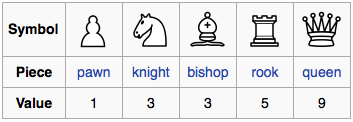
\includegraphics{Chess_piece_relative_value.png}
  \caption{Chess piece values  \label{fig:chessPieces}}
\end{figure}

\subsection{Network Play}

The specification demands that the game can play with other games over a network, this section describes the requirements for this. The specification does not give much detail on how this is to be achieved, so this section makes several assumptions that must be agreed with the customer.

\begin{table}[H]
\caption{Network  requirements}
\label{table:networkReqs}
\begin{tabular}{|| l | p{10.5cm}  |  c  | c ||} \hline  
% BE REALLY carefull with this, it contains pipe symbol | and lower case l (L), make sure you are clear which is which before you change anything
\textbf{Number} & \textbf{Requirement} & \textbf{Source} & \textbf{Priority}\\ \hline

\textbf{REQ-Net1:}  & The game must allow finding a network player from a given IP& Spec & \textit{ High} \\

\textbf{REQ-Net2:} &
The application opens IP Port 4567 when starting and closes it when it exits  (for network play)
& Spec  &  \textit{High}\\

\textbf{REQ-Net3:} &
The network play only needs to work on the same subnet, no IP routing across routers or firewalls is needed. 
& Interview  &  \textit{High}\\

\textbf{REQ-Net4:} &  
Active mode: The game starting a network game is said to be in Active network mode
& Derived  &  \textit{High}\\

\textbf{REQ-Net5:} &  
Active mode: If the user selects Network Game at game start, the application will ask for an IP address of another game.
& Spec  &  \textit{High}\\

\textbf{REQ-Net6:} &  
Active mode: Once an IP address is entered, the game will attempt to contact and connect to a game at that address.
& Derived  &  \textit{High}\\

\textbf{REQ-Net7:} &  
Only IP V4 will be used, no IP V6 support.
& Derived  &  \textit{Medium}\\

\textbf{REQ-Net8:} &  
Active mode: IP addresses will be entered the normal format of xxx:xxxx:xxxx:xxxx where each xxxx represents a 8 bit value in decimal notation, for example 192.168.135.33
& Derived  &  \textit{Medium}\\

\textbf{REQ-Net9:} &  
Active mode: If no response is received from the given IP address in a defined time, an error is displayed and the game state reverts to game-not-started. & Derived  &  \textit{High}\\

\textbf{REQ-Net10:} &  
Active mode: The time-out will be a system global constant in the first release, and is not user configurable
& Derived  &  \textit{Low}\\

\textbf{REQ-Net11:} &  
Passive Mode: The game waiting to receive a network play partner id said to be in Passive mode.
& Derived  &  \textit{High}\\


\textbf{REQ-Net12:} &  
Passive Mode: At game start, the user can select Network game, Passive mode
& Derived  &  \textit{High}\\


\textbf{REQ-Net13:} &  
Passive Mode: The game will wait indefinitely for an incoming connection request on port 4567.
& Derived  &  \textit{High}\\


\textbf{REQ-Net14:} &  
Passive Mode: The user can cancel passive mode and return to the game-not-started state.
& Derived  &  \textit{High}\\


\textbf{REQ-Net15:} &  
Passive Mode: Once a connection is opened, the Active game sends player details, and the Passive game also responds with player details.
& Derived  &  \textit{High}\\


\textbf{REQ-Net16:} &  
After that, moves are exchanged until the game is complete or either played selects 'Stop Game'.
 & Derived  &  \textit{High}\\


\hline
\end{tabular}
\end{table}

\subsection{User Interface }
<<<<<<< HEAD
%\todo{Mohamed Khaliqi - add wireframes here}
=======



>>>>>>> 6814dc6a329b348e7ef9c0ed8e5bf7fc631eafc1
In this Section, A demonstration of the software will be shown as below. In order to have Mock up, we used JAVA and JFC and Swing GUI\footnote{The hard code of this demo is available if it is needed.}. According to Walrath, Kathy \footnote{The same article is also available in Java JFC and Swing tutorial in Oracle website : \url{http://docs.oracle.com/javase/tutorial/uiswing/start/about.html}} ``JFC is short for Java Foundation Classes, which encompass a group of features for building graphical user interfaces (GUIs) and adding rich graphics functionality and interactivity to Java applications. It is defined as containing the features shown in the table below.'' and Swing ``Includes everything from buttons to split panes to tables. Many components are capable of sorting, printing, and drag and drop, to name a few of the supported features. '' \cite{walrath2004jfc} \\

\begin{figure}[h]
  \centering
	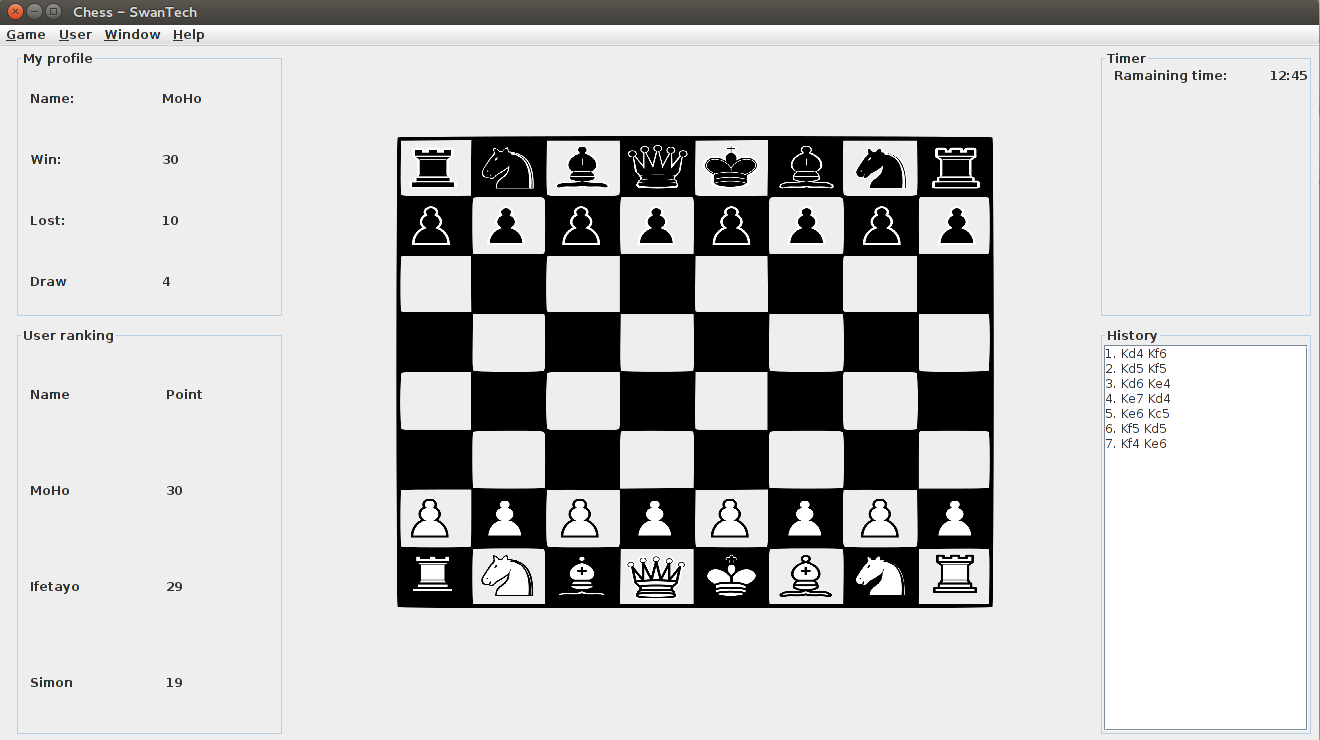
\includegraphics[width=\textwidth]{WholeApp.png}
  \caption{Whole interface will all panels}
  \label{fig:wholeapp}
\end{figure}
Above figure shows all aspect of the application. Menus, panels and board in the middle of the screen. The final project will be very similar to this figure.
\clearpage
\pagebreak
\begin{figure}
  \centering
	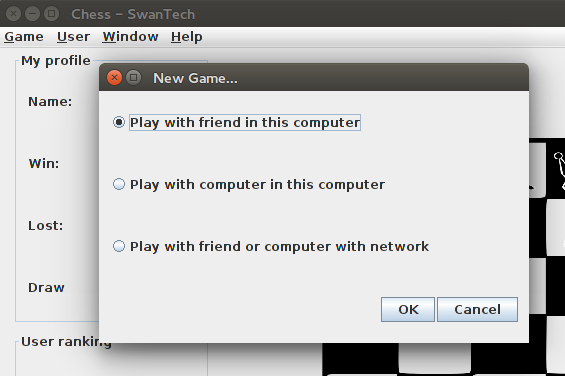
\includegraphics[width=\textwidth]{NewGame.png}
  \caption{New game dialog  \label{fig:newgamedialog}}
\end{figure}
In this figure, when user try to start a new game, a dialog with three options comes to the screen and user should choose the type of game. The default option is play with friend in the curent computer. Depends on user choice the type of game will change.  
\clearpage
\pagebreak
\begin{figure}[!htb]
\minipage{0.45\textwidth}
  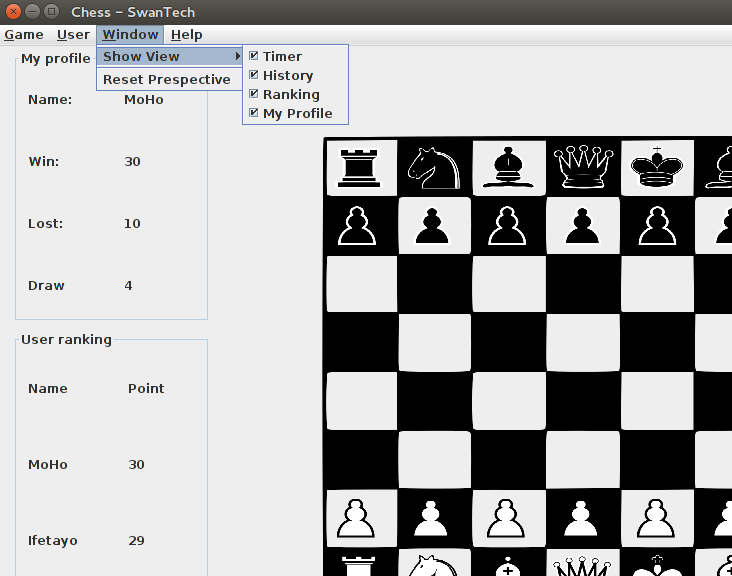
\includegraphics[width=7cm]{Menu.png}
  \caption{Available menu  \label{fig:menu1}}
\endminipage\hfill
\minipage{0.45\textwidth}
  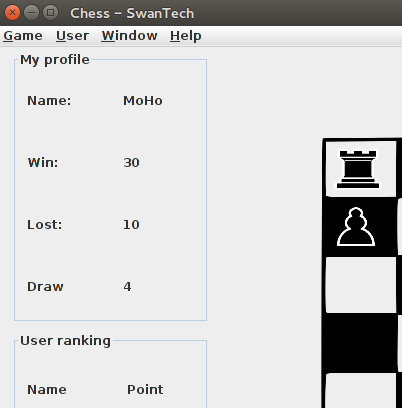
\includegraphics[width=6cm]{Menu2.png}
  \caption{Sub Menus with functionality  \label{fig:menu2}}
\endminipage\hfill
\end{figure}
These two pictures demonstrate the menu with functionality to show or hide panels in the program. They are all written by Swing and JMenu, JMenuItem and JCheckBoxMenuItem methods. There are also Mnemonic and Accelerator for necessary items in menu like shotcut key Ctrl+N is assigned for new game or Alt+G is for \textit{Game menu} and so on. 

\begin{comment}
\begin{figure}
  \centering
	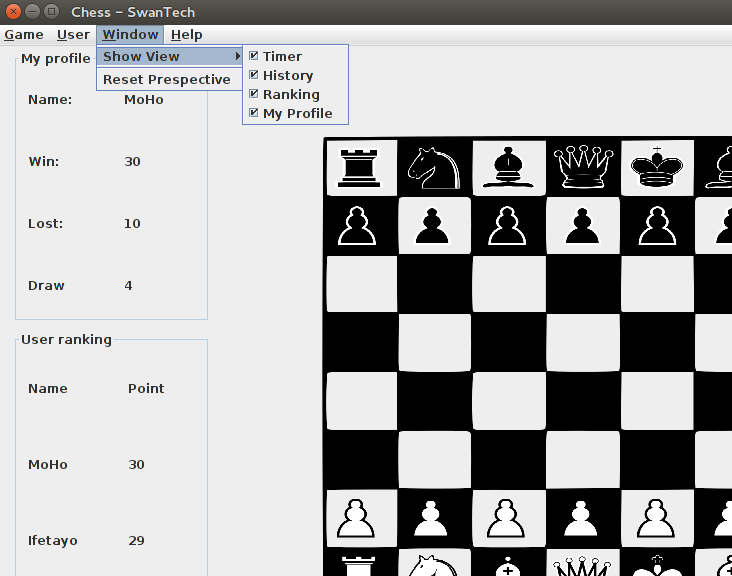
\includegraphics[width=7cm]{Menu.png}
  \caption{Available menu  \label{fig:chessPieces}}
\end{figure}

\begin{figure}
  \centering
	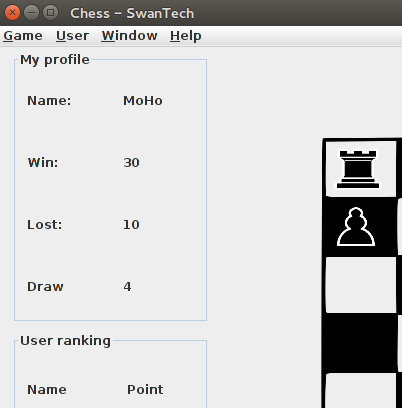
\includegraphics[width=7cm]{Menu2.png}
  \caption{Sub Menus with functionality  \label{fig:chessPieces}}
\end{figure}
\end{comment}
%-----------------------------------------------------------------------------------------
% Design secition
%-----------------------------------------------------------------------------------------
\section{System Design}

\subsection {Class Structure}


\subsection {UML Collaboration Diagram}
\subsubsection{Activity Diagram}
According to Booch, Grady ``Activity diagrams are graphical representations of workflows of stepwise activities and actions with support for choice, iteration and concurrency. In the UML, activity diagrams are intended to model both computational and organisational processes. Activity diagrams show the overall flow of control.''\cite{booch1999uml}\\
In this diagram(next page), some part of the system has been broken to \textit{Call Activity Nodes} because of limit space in the page. First one on top, is about how to uncheck when the player is check. Second one, explain why a piece might be impossible to move. Next one is all possible movement and the last one is when a player is check and how can player should react when it is checked. To uncheck(if it is possible), the first call activity node is solution.
\clearpage
\pagebreak
\begin{figure}
  \centering
	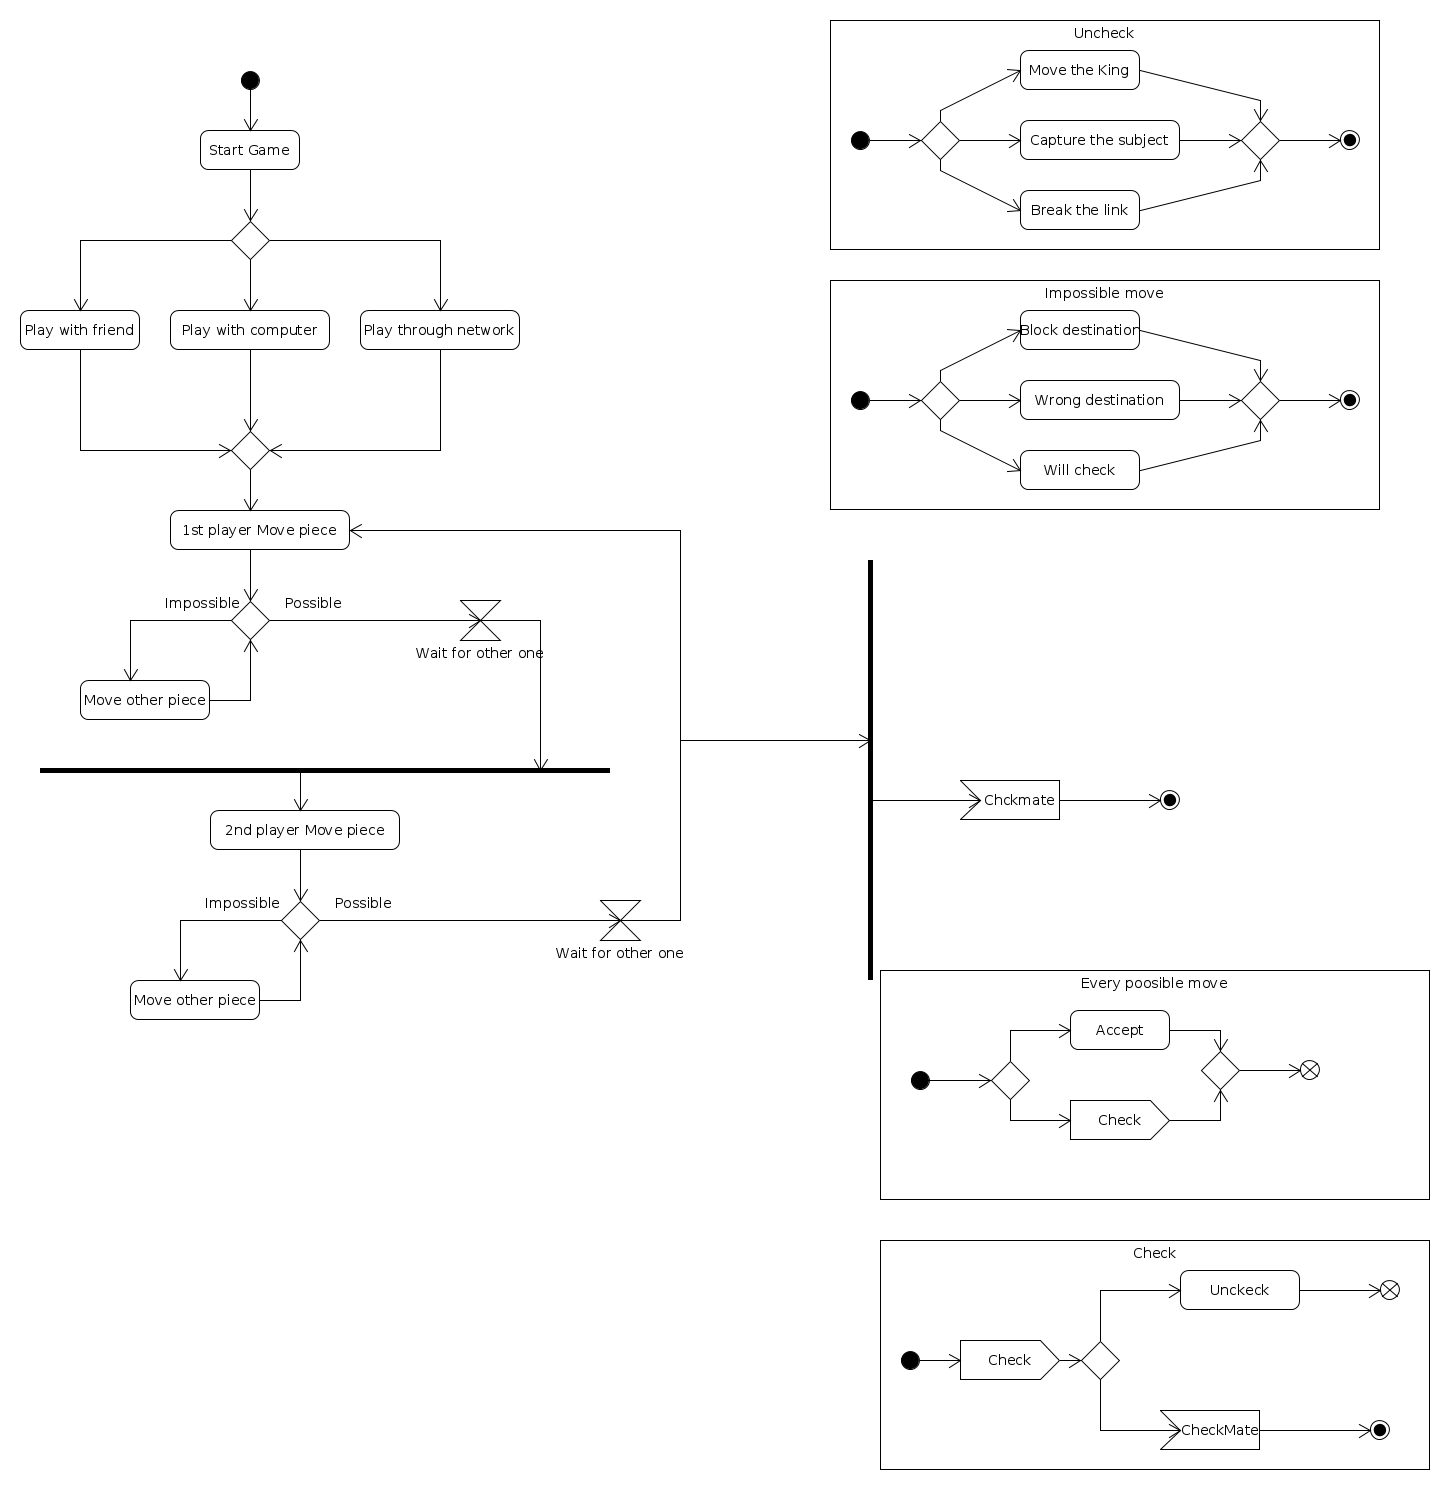
\includegraphics[width=\textwidth]{activitydiagram}
  \caption{Project Activity Diagram  \label{fig:activitydiagram}}
\end{figure}
\clearpage
\pagebreak
%-----------------------------------------------------------------------------------------
% Other Non-functional Requirements
%-----------------------------------------------------------------------------------------
\section{Other Non-functional Requirements}

\subsection{Technical Environment}
This section describes the direct technical environment requirements derived from the specification.



\begin{table}[H]
\caption{Non Functional  requirements}
\label{table:NFReqs}
\begin{tabular}{|| l | p{10.5cm}  |  c  | c ||} \hline  
% BE REALLY carefull with this, it contains pipe symbol | and lower case l (L), make sure you are clear which is which before you change anything
\textbf{Number} & \textbf{Requirement} & \textbf{Source} & \textbf{Priority}\\ \hline
\textbf{REQ-NF1:}  & The application must be runnable on Phones, Tablets and Computers & Spec & \textit{ High} \\

\textbf{REQ-NF2:} 
&  The game does not have to run on IOS devices
& Interview  &  \textit{High}\\

\textbf{REQ-NF3:} 
&  The game will run on Android tablets and phones
& Derived  &  \textit{High}\\

\textbf{REQ-NF4:} 
&  The game will run on Windows and OS X PCs provided they can host the appropriate JVM
& Interview  &  \textit{High}\\


\textbf{REQ-NF5:} 
& It will be possible to use an alternative Chess Engine. It may be that a Java class has to be subclassed and modified to make this possible. 
& Interview  &  \textit{High}\\

\hline
\end{tabular}
\end{table}


\subsection{Performance Requirements}

Many aspects of the game performance are beyond the control of the software team, such as:
\begin{itemize}
  \item The performance of the device, from Phones to PCs
  \item The performance of the network
  \item The performance of the Chess engine
\end{itemize}

So we will give only limited assurances on performance. 

\begin{table}[H]
\caption{Performance  requirements}
\label{table:PerfReqs}
\begin{tabular}{|| l | p{10.5cm}  |  c  | c ||} \hline  

\textbf{Number} & \textbf{Requirement} & \textbf{Source} & \textbf{Priority}\\ \hline

\textbf{REQ-NF20:}  & 
The application will start and load its persistent data within 20 seconds
& Spec & \textit{ High} \\

\textbf{REQ-NF21:} 
&  From selecting a piece, legal moves will be displayed within 5 seconds
& Interview  &  \textit{High}\\

\textbf{REQ-NF22:} 
&  From selecting a legal move, the other player move can commence within 5 seconds.
& Derived  &  \textit{High}\\

\hline
\end{tabular}
\end{table}


\subsection{Safety Requirements}

We can foresee no direct safety concerns in the application. Clearly as with all other computer games, they should not be used while driving or operating machinery. 

\subsection{Security Requirements}

Within the limitations of a 10 unit module, particularly when we have only three team member for a project designed for five, we have decided that we will not implement any security requirements, and in particular:

\begin{itemize}
\item No user password will be required to play the game
\item Game moves will be sent over the network in plaintext, including player names, profiles and scores
\item No action will be undertaken to verify the identity of a remote network player
\item Persistent player data will be stored in plaintext
\end{itemize}

We believe that as the game does not involve any payment and requires no personal detail, this is acceptable. Furthermore, network play is limited by the span of a local area network so it is unlikely that a player will really be able to play with another 'anonymous' player but will be someone they know or how is in sight.

If the game were extended to a Internet enabled game, these limitations would not be acceptable. 

\subsection{Software Quality Attributes}

The project will of course strive for a high standard of software quality. The tools we will use to achieve this are:


\begin{itemize}
  \item The class design will support isolation of concerns, loose coupling and adaptability. 
  \item Conformance with    'Bob’s Concise Coding Conventions (C3 )' \cite{bobsccc} will ensure the readability and help drive the reliability of the code.
\item Doxygen will create the software documentation, this makes it easier to ensure the software and the docs are aligned.
\item The team will perform peer code reviews on all code and verify the Doxygen documentation is correct.
\item The test manager will review all test classes and check they are adequate to ensure a quality software delivery. 
  \item Each of the team will develop unit test classes along with the classes that they are allocated for development.
\item A complete unit and interface test suite will be developed and run as part of the build cycle. 
\item Using Git and GitHub helps  manage concurrent development and safe commit points. 
\item A RDA development approach will ensure we converge on the customers real requirements and will enable us to identify the choke points early on in the development. 
\item Focus will be on usability and completeness, if necessary at the expense of attributes such as availability and correctness. 
\end{itemize}



%-----------------------------------------------------------------------------------------
% Appendices
%-----------------------------------------------------------------------------------------
\begin{appendices}
\section{Glossary}

\newglossaryentry{Linux}
{
  name=Linux,
  description={is a generic term referring to the family of Unix-like
               computer operating systems that use the Linux kernel},
  plural=Linuces
}

\newglossaryentry{Windows}
{
  name=Windows, 
  description={is a proprietary OS  from Microsoft\textregistered},
}

\newglossaryentry{OS X}
{
  name=OS X,
  description={The proprietary OS from Apple\textregistered{} used on Imacs\textregistered{}  and MacBooks\textregistered. Based on  BSD Unix.},
}

\newglossaryentry{OS}
{
  name=OS,
  description={Operating System, the software that makes a PC or device work.},
}

\newglossaryentry{UCI}
{
  name=UCI,
  description={Universal Chess Interface, is an open communication protocol that enables a chess program's engine to communicate with its user interface},
}

\newglossaryentry{TCP/IP}
{
  name= TCP/IP,
  description={Transmission Control Prototcol / Internet Protocol, the standard protocol of the Internet},
}

\newglossaryentry{IOP}
{
  name=IP,
  description={See TCP/IP},
}


\newglossaryentry{PNG}
{
  name=PNG,
  description={Portable Game Notation, see references},
}




\printglossaries
\glsaddall


\section{To Be Determined List \label{TBDList}}
\begin{enumerate}
  \item Use UIC or PNG for exchanging Chess move data
\item Choice of Chess engine
\end{enumerate}


\section {Team Minutes}
   \lstset{language=C++,
           basicstyle=\ttfamily,
           keywordstyle=\color{blue}\ttfamily,
           stringstyle=\color{red}\ttfamily,
           commentstyle=\color{green}\ttfamily,
          breaklines=true
          }
\begin{lstlisting}[frame=single,caption=Meeting of 9/2/15,label=minutes1]


Minutes of Meeting 2: Simon, Ifetayo, Mo, David
-----------------------------------------------
Date: 9th Feb 2015
Start: 15:02
End: 15:51

Next Meeting: 11th Feb 12:00

Topics Discussed:
-- Group name decided upon = SwanTech
-- Team roles discussed based on strengths and preference. 
	Simon = Customer Interface Manager
	David = Design Manager
	Ifetayo = Implementation Manager
	Mo = Test Manager
	Planning & Quality Manager = Unassigned and therefore split between
	 members.
-- Discussed familiarity with software, programming languages and applicable services
   such as Latex, Java and GitHub. Also considered tutorials to aid with any unfamiliarity. 
-- Programming software to be used and compared as part of project =  NetBeans vs. Eclipse.

Progress Since Last Meeting:
-- Facebook group setup to aid communication and organisation.
-- Shared area set up on blackboard for file storage.
-- Minute and coding convention guidelines read.

TODO:
-- Mo = Check JUnit test framework for full testing capability including GUI.
      = Set up GitHub account and share tutorial links.
-- Simon = Check with client whether Latex is a requirement or recommendation for project.
	 = Skeleton for next assignment.
-- David = View tutorials and get acquainted with Latex and Java programming software.
	 = Collate team contributions into document for submittal.
-- Ifetayo = Investigate which version of java will be used and program for project 
   management(Gantt Chart).
-- ALL = Ensure relavent software is installed and updated.
       = Read Doxygen introduction.
       = Write page on what each member expects to be doing when project is given including an
	 outline of sections which each member feels needs to be part of the projects documentation.
	 SEND TO DAVID BY MONDAY 16TH!!
\end{lstlisting}

\begin{lstlisting}[frame=single,caption=Meeting of 11/2/15,label=minutes2]
Minutes of Meeting 2: Simon, Ifetayo, Mo, David
-----------------------------------------------
Date: 11th Feb 2015
Start: 11:50
End: 12:00

Next Meeting: 16th Feb 15:00

Topics Discussed:
-- Decided to use Latex for the project write up.
-- Discussed the use of project management suite visual studio online.
-- Pages of report coming along well.

Progress Since Last Meeting:
-- Possible template for project found.
-- GitHub for the group set up.

TODO:
-- All = Complete pages for report.
       = Finish any other tasks set from previous meeting.
       = Think about timeline/activity schedule to be followed when project specifications given.

\end{lstlisting}

\begin{lstlisting}[frame=single,caption=Meeting of 16/2/15,label=minutes3]

Minutes of Meeting 3: Simon, Ifetayo, Mo, David
-----------------------------------------------
Date: 16th Feb 2015
Start: 15:03
End: 15:22

Next Meeting: 18th Feb 12:00

Topics Discussed:
-- Mo found a plugin for eclipse which allows testing of GUI and other plugins to aid code quality namely PMD and CodePro Analytix.
-- Discussed how the code repository is to function in relation to errors and branches.
-- Submittal process for the assignment.
-- Setting up visual studio online for project management.

Progress Since Last Meeting:
-- Completed pages for assignment report.
-- Decided upon Java version.
-- Facebook issues resolved.
-- Doxygen notes read.

TODO:
-- Mo + David = Final additions and tweaks to assignment before everyone submits.
-- All = Set up microsoft accounts for using visual studio online.
       = Submit the assignment by Wednesday 18th 11:00.


\end{lstlisting}

\begin{lstlisting}[frame=single,caption=Meeting of 23/2/15,label=minutes4]

Minutes of Meeting 4: Simon, Ifetayo, Mo
-----------------------------------------------
Date: 23th Feb 2015
Start: 15:00
End: 15:30

Next Meeting: 25th Feb 12:00

Topics Discussed:
-- Assignment part 2 released and discussed. Task - design a Chess program
-- Open issues and questions - SH to discuss with Dr Mora (arranged Tuesday 24 16:00)
-- SH to create issues log etc
-- Ifetayo suggested we all bring initial design ideas on Class structure to Wednesday lecture
-- SH to set up requirements spec

Progress Since Last Meeting:
-- Assignment 1 submitted on time

TODO:
-- All = Set up microsoft accounts for using visual studio online.
-- SH to set up meeting with Dr Mora, and request extension (done)
-- Initial Class design ideas by Wednesday

Questions for Dr Mora

What devices do we need to run on - can we exclude IOS & OS X?
Assuming Java - hence problems with IOS & OS X
Is a web only solution acceptable?
Android, do we need to supply APK file?
Who will sign off the requirements?
Clarify `Computer Human Network`
Device to device - same subnet?
Ports blocked at Swansea?

\end{lstlisting}

\begin{lstlisting}[frame=single,caption=Meeting of 26/2/15,label=minutes5]

Minutes of Meeting 5: Simon, Ifetayo, Mo
-----------------------------------------------
Date: 26th Feb 2015
Start: 13:10
End: 14:20

Next Meeting: 2nd Mar 15:00

Topics Discussed:
-- Discussion from Dr.Mora`s course work feedback
--- Course work part 2 Specification and Design Document discussed 
--- Update on open issues and questions from last meeting
--- Feedback from Simon on meeting with Dr.Mora
--- Discussion of individual class diagrams (Identification of the objects)
--- Best way to go about the development of the project (web maybe?)
-- Chess engine is to be run local on each instance of the app
-- Simon has come up with a template for the team`s documentation. No user documentation and security requirements, additional sections are to be added as appilicable
-- Unicode characters for the chess pieces can be used for documentation
-- Latex is to be used for all documentation purposes

Progress Since Last Meeting:
-- Ambiguities from the requirement documentation have been clarified
-- No IOS development is to be done

TODO:
-- Ifetayo is to design the class diagram and use cases
--- Simon is to draft the project requirements and design the state chart
--- Mo is to design the UML, Mock up, logo, convert the teams agreed document template to latex and document the state chart design from Simon
-- Movelist feature is to be of low priority
-- Persisting data is to be done however the member handling it decides
-- Doxygen generation of class diagram using Argo or doxygen is to be investigated by Mo


Questions for next meeting

What technology or approach is suitable for the project implementation
Other language possibilities

\end{lstlisting}

\begin{lstlisting}[frame=single,caption=Meeting of 2/3/15,label=minutes6]

Minutes of Meeting 6: Simon, Ifetayo, Mo
-----------------------------------------------
Date: 2nd March 2015
Start: 13:00
End: 14:00

Next Meeting: 9th Mar 15:00

Topics Discussed:

--- Ifetayo`s class diagram discussed at length. SH & MK to read and comment
--- Wire Frame interface layout - Mo to produce soon.
--- Requirements - complete, to be reviewed.


Progress Since Last Meeting:
--- latex software development spec complete and partly populated
--- Class diagram 1st draft complete

TODO:
-- Ifetayo is to complete design the class diagram and use cases
--- Simon is to design the state chart
--- Mo is to design the UML, Mock up, logo, 
-- Persisting data is to be done however the member handling it decides
-- Doxygen generation of class diagram using Argo or Doxygen is to be investigated by Mo

\end{lstlisting}

\begin{lstlisting}[frame=single,caption=Meeting of 9/3/15,label=minutes7]

Minutes of Meeting 7: Simon, Ifetayo, Mo
-----------------------------------------------
Date: 9th March 2015
Start: 13:00
End: 13:30

Next Meeting: 16th Mar 15:00

Topics Discussed:

 Ifetayo`s class diagram agreed.
--- Wire Frame interface layout - Mo produced, look good.
--- The wire frame are produced in Java. We agreed the Java source will be available on
      GitHub for examination if desired. 
--- SH agreed to complete remaining unallocated sessions.
--- Ifetayo will insert Class Diagrams into latex before Wednesday
--- All on target for deadline



Progress Since Last Meeting:
--- Class diagrams, requirements, class diagrams, UML all complete
--- Report on target for deadline Wednesday 11/3/15

TODO:
-- Ifetayo is to complete design the class diagram and use cases and add to LaTex doc 
 Mo is to add the UML, Mock up, logo, to report

\end{lstlisting}




\clearpage
\pagebreak
\section{References}
\bibliography{Assignment_2}{}
\bibliographystyle{ieeetr}

\end{appendices}
\end{document}
